% easychair.tex,v 3.1 2011/12/30
%
% Select appropriate paper format in your document class as
% instructed by your conference organizers. Only withtimes
% and notimes can be used in proceedings created by EasyChair
%
% The available formats are 'letterpaper' and 'a4paper' with
% the former being the default if omitted as in the example
% below.
%
\documentclass[procedia]{easychair}
\usepackage{amsmath}
%\documentclass[debug]{easychair}
%\documentclass[verbose]{easychair}
%\documentclass[notimes]{easychair}
%\documentclass[withtimes]{easychair}
%\documentclass[a4paper]{easychair}
%\documentclass[letterpaper]{easychair}

% This provides the \BibTeX macro
\usepackage{doc}
\usepackage{makeidx}
\usepackage{subfig}

% In order to save space or manage large tables or figures in a
% landcape-like text, you can use the rotating and pdflscape
% packages. Uncomment the desired from the below.
%
% \usepackage{rotating}
% \usepackage{pdflscape} 

% If you plan on including some algorithm specification, we recommend
% the below package. Read more details on the custom options of the
% package documentation.
%
% \usepackage{algorithm2e}

% Some of our commands for this guide.
%
\newcommand{\easychair}{\textsf{easychair}}
\newcommand{\miktex}{MiK{\TeX}}
\newcommand{\texniccenter}{{\TeX}nicCenter}
\newcommand{\makefile}{\texttt{Makefile}}
\newcommand{\latexeditor}{LEd}

\def\procediaConference{99th Conference on Topics of
  Superb Significance (COOL 2014)}

%\makeindex

%% Front Matter
%%
% Regular title as in the article class.
%
\title{Multiscale and Multiresolution methods for  \\
Sparse representation of Large datasets  }

% \titlerunning{} has to be set to either the main title or its shorter
% version for the running heads. When processed by
% EasyChair, this command is mandatory: a document without \titlerunning
% will be rejected by EasyChair

\titlerunning{A Guide for Writing \LaTeX\ Documents \ldots}

% Authors are joined by \and. Their affiliations are given by \inst, which indexes into the list
% defined using \institute
%
\author{
    Prashant Shekhar\inst{}%\thanks{Designed and implemented the class style}
\and
    Abani Patra\inst{}%\thanks{Did numerous tests and provided a lot of suggestions}
\and 
    Beata M. Csatho
\\
}

% Institutes for affiliations are also joined by \and,
\institute{
  State University of New York at Buffalo, New York, U.S.A\\
  \email{pshekhar@buffalo.edu, abani@buffalo.edu, bcsatho@buffalo.edu}
%\and
%  State University of New York at Buffalo, New York, U.S.A\\
%  \email{abani@buffalo.edu}\\
 }
%  \authorrunning{} has to be set for the shorter version of the authors' names;
% otherwise a warning will be rendered in the running heads. When processed by
% EasyChair, this command is mandatory: a document without \authorrunning
% will be rejected by EasyChair

\authorrunning{Shekhar and Patra}

\begin{document}

\maketitle

\keywords{Multiscale,Multiresolution,Kernel methods, Sparse representation}

\begin{abstract}
In this study, we have presented a strategy that aims at studying an observational dataset at different resolutions to obtain a sparse representation in a computationally efficient manner. Resolution here stems from the variation of the correlation strength among the different obser- vation instances. The idea behind the approach is to make a large dataset as small as possible by removing all the redundant information so that as per the requirement, the original data could be reconstructed with minimized losses of information. We have tested our approach on a carefully designed suite of analytical functions along with gravity and altimetry time series datasets from a section of the Greenland Icesheet. Besides providing a good strategy for data compression, the proposed approach also finds application in efficient sampling procedures and error filtering in the datasets. The results presented in the article clearly establish the promis- ing nature of the approach along with prospects of its application in different fields of data analytics in the scientific computing as well as other related domains
\end{abstract}

%\setcounter{tocdepth}{2}
%{\small
%\tableofcontents}

%\section{To mention}
%
%Processing in EasyChair - number of pages.
%
%Examples of how EasyChair processes papers. Caveats (replacement of EC
%class, errors).


%------------------------------------------------------------------------------
\section{Introduction}
\label{sect:introduction}

The disproportionate increase in the volume of the data in scientific observations and modeling and limitations in computational resources has motivated research in new ways of data compression and learning for converting that data to information. The multiscale and multiresolution methodology proposed in this paper directly follows from our previous work \cite{patra2016multilevel} and exploits the correlation structure inherent in the dataset and uses this information to compress the dataset to a reduced number of observation instances while minimizing the information loss. The related problem of data compression has been a crucial tool in several fields like image compression \cite{rufai2014lossy} and various techniques like signal processing have contributed well to this approach of analyzing data  \cite{sandryhaila2014big}. We focus here on obtaining sparse representations of spatio-temporal datasets where proximity in time and/or space makes reasoning about correlation structures much easier. This approach by its very nature is relevant for a variety of data science domains but we focus here on data from gravity and altimetry of a section of the Greenland Icesheet. Data analytics and data handling approaches have also been widely used in science related domains. Like for example \cite{guan2016inferring} presented a bayesian approach where they have integrated various datasets with a Glacier dynamics model for inferring icesheet thickness in Western Antarctica

Besides being a data compression approach, the proposed methodology can also be thought of as an efficient sampling method for analyzing high volume outputs of various numerical and data driven models. This could be understood as follows. Suppose we wish to generate the velocity profile of some fluid over a land area for which we already know the topography profile represented by a digital elevation model(DEM). Then based on the sparse representation of the DEM, we can approximately locate the critical locations over that land area which can represent the entire variability in the topography with missing locations quickly computed by an interpolatory process with minimal error. Therefore, if we can get velocity measurements over those critical coordinates, we can get a very good approximation of how the DEM would affect the velocity profile over the area without incurring much error or cost through unnecessary measurements. Thus it also leads to an indirect filtering of errors which might creep in due to large number of measurements. In an approach related to this, Chatterjee and colleagues \cite{chatterjee2013adaptive} used neural networks for filtering and compression of their biomedical dataset.

A singular challenge in these methods is the accurate representation of data with rapid changes. In the literature on finite elements and other modeling methods, researchers have for long been trying to develop efficient procedures for capturing of discontinuities. In this regard it is relevant to refer to the Extended Finite Element method \cite{NME:NME726}  which proposed a solution based on enriching the basis functions used for approximation by including several discontinuous functions. The proposed approach can also be thought of as an efficient way to generate basis functions which can efficiently model such rapid changes by optimal exploitation of correlation structures inherent in the data at different scales and resolutions. The exact meaning of scales and resolution with reference to the proposed procedure will be discussed in detail in the following sections.

Besides testing the approach on a set of analytical functions \cite{simulationlib}, we have also analyzed the procedure on two sets of time series data for the gravity measurements \cite{luthcke2013antarctica} and the altimetry measurements \cite{schenk2012new} at critical locations on the surface of the greenland icesheet. This dataset is a crucial parameter for the performance of our algorithm because of the high fluctuations inherent in this data. Also, the application on this dataset clearly brings out the capability of our approach to remove unnecessary noise from the information built into the data.

The contributions of this paper can be summarized as follows. Firstly, we are introducing methods for sparse representation which analyze the inherent structure of the dataset and remove redundant information which is beneficial for memory savings and efficient computations. Secondly, unlike previously, here we are using a composition of scales and resolutions which represents the levels and sublevels at which a dataset can be studied. Due to this capability we are even able to model rapid changes through efficient basis construction.



%------------------------------------------------------------------------------


\section{Multiscale/Multiresolution approach with Kernels }
\label{sect:approach}

Bermanis and co-workers \cite{bermanis2013multiscale} developed approaches to sampling from a dataset at different scales to build efficient interpolators. In previous work \cite{patra2016multilevel}, building on this foundation we introduced multigrid inspired methodology to develop efficient sparse representations of datasets and illustrated it with application to topographies. The approach as discussed in our previous work \cite{patra2016multilevel} is based on a QR matrix decomposition procedure which identifies the observation instances with maximum amount of information (through the decomposition of the covariance kernel) and uses them along with the kernel specified as a sparse representation for the original dataset. Then this sparse representation could be used to predict the original function at any time as required. The application of the approach has been shown on 4 analytical functions along with two real datasets from the geophysical domain.
This approach fundamentally relies on a good characterization of the correlation structure. Our previous work relied completely on the classical squared exponential kernels to represent the covariance (\ref{1}). While, this kernel does correctly capture the spatial dependence of many data sets using the parameter ε to choose the scale and allows multiscale representations (see \cite{rasmussen2006gaussian} for details) there are many other data sets for which this is not the best choice.


\begin{equation}
g_\epsilon (r) = exp\left({-\frac{r^2}{\epsilon}}\right)
\label{1}
\end{equation}

For the current work, we examine a rational quadratic kernel that allows us to capture more general covariance structure by manipulating both the length scale and an additional resolution parameter $\alpha$ (\ref{2}). Here r represents the distance between two observation points through an appropriate metric and $\epsilon$ represents a length scale similar to the square exponential kernel shown in (\ref{1}). The term $\alpha$ here represents the second variable which also allows us to vary the behavior of the covariance kernel. The presence of two scale parameters in the kernel expression ($\epsilon$ and $\alpha$) enables it to have a mixture of scales and resolutions for different points in the domain.


\begin{equation}
k_{RQ}(r) = \left({1 + \frac{r^2}{2 \alpha \epsilon^2}}\right)^{-\alpha}
\label{2}
\end{equation}

Thus, through the use of the rational quadratic kernel our approach is able to study and model the data by studying the behavior of the data at different scales (variation of $\epsilon$) and then adaptively varying the resolution ($\alpha$) at each scale in order to have a higher accuracy at critical points (for example at a discontinuity). The squared exponential on the other hand is limited only to the choice of the length scale.

%______________________________________________________________
\section{Sparse Representation}
\label{sect:sparse}

The idea of sparse representation introduced in this work is suppose to target the need of data compression and optimal storage for a given large dataset. Data compression has been a well explored topic in the recent past. \cite{liu2014self} discussed it with respect to image classification. \cite{yang2011learning} have implemented this concept in reference to classification problem. In the current approach, we are not reducing the size of the given data by compressing the dimensions. Our data compression is based on reducing the number of observations itself by decimating data with minimal information content. Conceptually, the process aims to remove the observations from the dataset which have negligible information contribution given other observation points. Our multiscale and multiresolution based approach achieves this objective of data compression by creating a new data structure which is a compressed representation of the original dataset. This data structure has 4 components- \{Representative data points in the original dataset; scale ID; resolution ID; Coordinates for the representative Basis functions\} .

Representative data points (also referred as  sparse representation) refer to the selected observations from the dataset. Scale ID here represents the scale value inbuilt into $\epsilon$ as shown in \cite{patra2016multilevel}. Resolution ID here is $\alpha$ (when $\alpha$ is assumed to be constant for the whole domain at each scale). The case for variable resolution ($\alpha$) has been discussed in the results section. The fourth component of this data structure refers to the weightage which needs to be given to the covariance values of the prediction points with respect to the representative points. Therefore for prediction at an unknown point, one just needs to find the covariance of this new point with respect to the representative points by using the scale id and the resolution id in the rational quadratic kernel and then doing a linear combination of these covariance values by using the coordinates as the weights.

\begin{figure}[]  % H because we want our figure to stay here
	\centering
	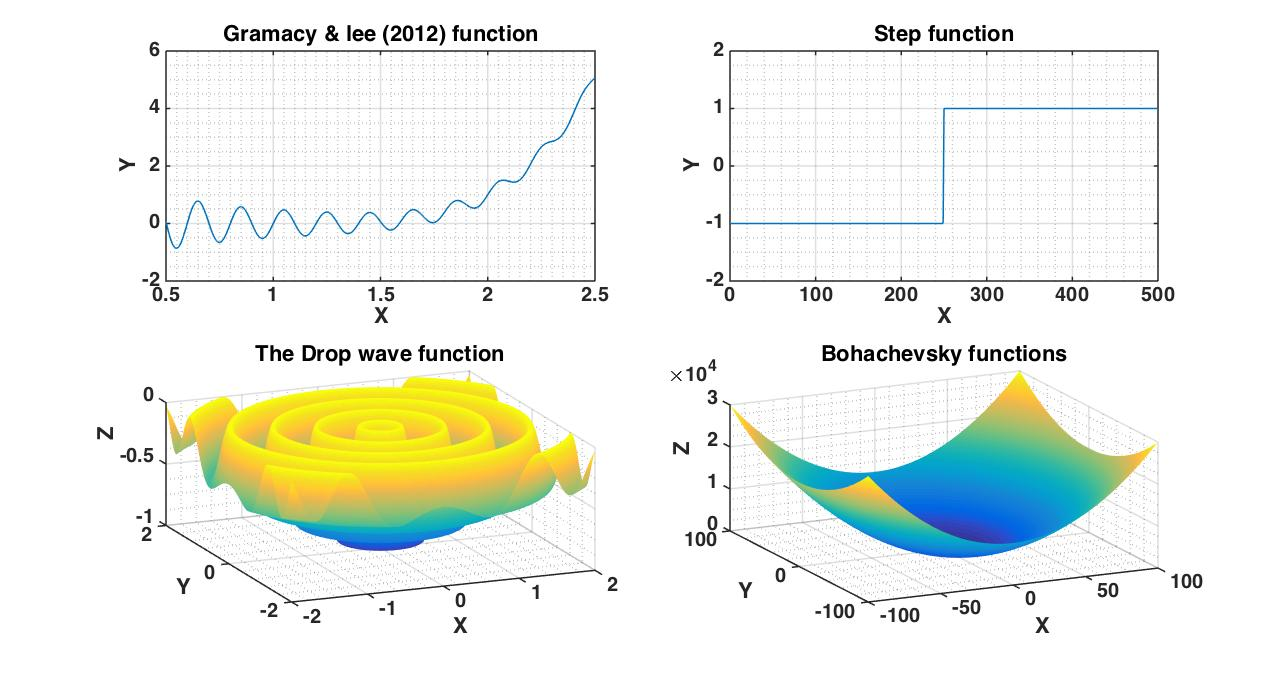
\includegraphics[width=4in]{plotfortest.jpg}
	\caption[Optional caption]{Test Functions}
	\label{fig1} %% for referencing the figure later on
\end{figure}


\section{Experimental setup}
In this section we have discussed our entire experimentation setup for the demonstration of the capabilities of our current approach. For the first part of the analysis we have generated the sparse representations for some of the carefully chosen analytical functions which can bring out the crucial properties of our approach. Each of these test functions have several characteristics which make them representative of a big class of practical cases. Each of these test functions would be specifically dealt with in the following part of the current section. 

We have also presented the results of the muli-scale and mlti-resolution approach on two datasets obtained from physical domains. The first dataset consists of NASA GSFC solution for monthly estimates of time-variable gravity in units of cm equivalent water height (cm w.e.) for a global set of 41,168 1x1 arc-degree equal-area mass concentration blocks.The  second dataset consists of Altimetry measurements over the surface of the icesheet at different locations over time. 

\subsection{Analytical Functions}

In this section, we will briefly go over all the test functions \cite{simulationlib} which we have used to demonstrate the performance of our approach. Figure \ref{fig1} shows the test functions used in this study to demonstrate the sparse representation generation capacity of our approach. Here compressed data representation refers to the procedure where we have some sampled points form an underly- ing function and then we carefully choose a minimal number of points which can represent the behavior pattern of the functions, thus minimizing the storage and computational resource requirement in the further analysis. The specific functions are:
 

%\begin{itemize}

%\item 1 dimensional function with global and local trends (Gramacy and Lee (2012) test function)
\begin{equation}
f(x)  = \frac{sin(10 \pi x)}{2x} + {(x-1)}^4
\label{3}
\end{equation}
%\item 1 dimensional function with a discontinuity (Step function)

\begin{equation}
f(x) = \left\{
        \begin{array}{ll}
            -1 & \quad x < 250 \\
            1 & \quad x \geq 250
        \end{array}
    \right.
\label{4}
\end{equation}


%\item 2 dimensional Multimodal function (The Drop Wave function)
\begin{equation}
f(x,y) = - \frac{1 + cos(12 \sqrt{x^2 + y^2})}{0.5 (x^2 + y^2)+ 2}
\label{5}
\end{equation}
%\item 2 dimension unimodel function (Bohachevsky function)
\begin{equation}
f(x,y) = x^2 + 2y^2 - 0.3cos(3 \pi x) - 0.4cos(4 \pi y) + 0.7
\label{6}
\end{equation}


%\end{itemize}

Here, (\ref{3}) represents a 1 dimensional function with global and local trends (Gramacy and Lee (2012) test function).(\ref{4}) has a speciality of a discontinuous function and will test the capability of the approach on sharp variations.The way in which our approach deals with the Gibbs phenomena of ringing at the discontinuity is also interesting to see. (\ref{5}) and (\ref{6}) are 2 dimension functions that are multimodal and unimodal respectively. These functions would gauge the performance in higher dimensions.



\subsection{Application to Observation Data}

The sparse representation generation for the mentioned analytical functions are meant to show if the algorithm is able to perform in an appropriate manner if the dataset is derived from a underlying function having a definite structure. Therefore, although these chosen functions are sufficiently complex based on their attributes, they lack the complexity level of a random dataset sampled from a physical domain because a practical dataset may even lack structure and may be even more difficult to model. 



\begin{figure}[]  % H because we want our figure to stay here
	\centering
	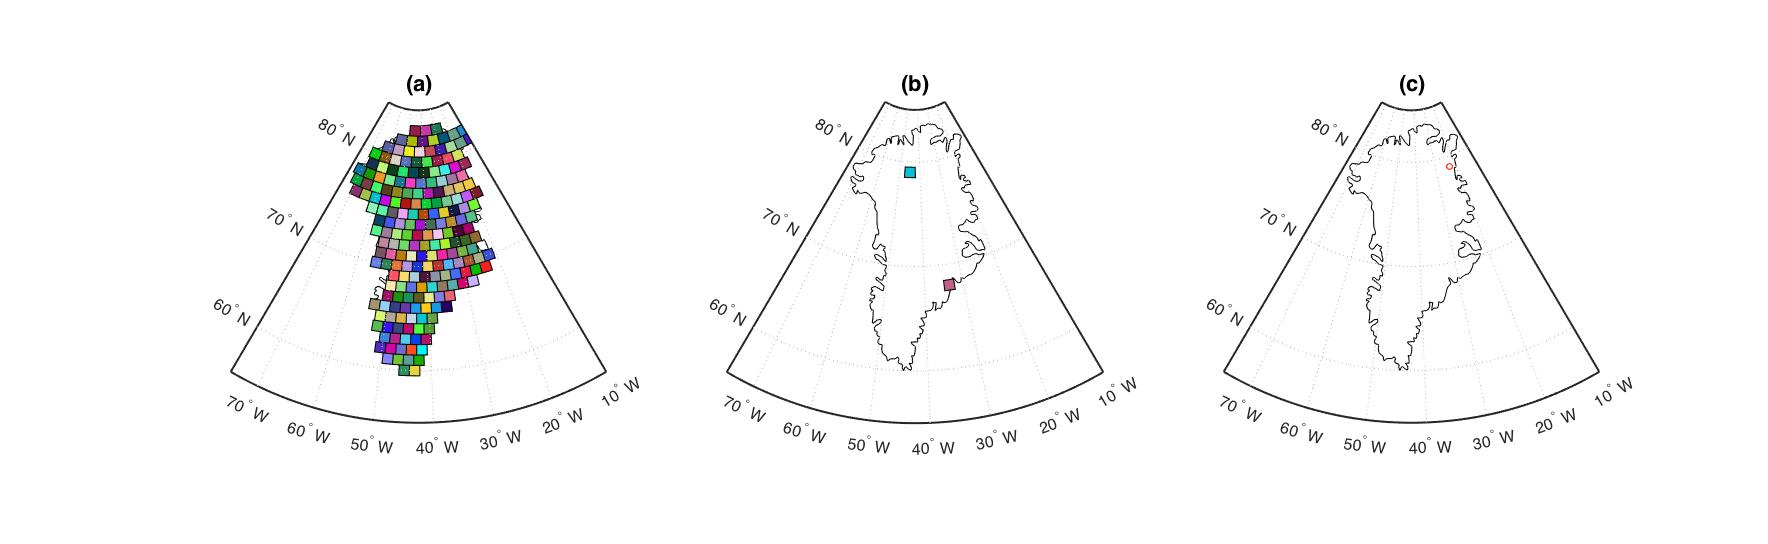
\includegraphics[width=5in]{grace_alt}
	\caption[Optional caption]{Gravity and Altimetry data a): Locations of all regions where Gravity time series is available b) The locations chosen for study c) Location of the coordinate (red circle in North East Greenland) for the time series of change in altimetry measurements }
	\label{fig2} %% for referencing the figure later on
\end{figure}

\subsubsection{Gravity Dataset}

Our first data is a gravity measurements dataset obtained from \cite{luthcke2013antarctica}. This dataset consists of 199 mascons (1x1 arc-degree equal-area mass concentration blocks or mascons) shown in the first figure in Figure \ref{fig2}. Each of these mascons have an associated time series of gravity measurements with them. This gravity data is in the form of monthly estimates of time-variable gravity in units of cm equivalent water height, which has been used as a proxy for the mass change measurements over the greenland icesheet. This data has been obtained after processing of the gravity measurements from the GRACE satellite mission. Since, this dataset consists of gravity measurements time series for each of the 199 mascons and each of these time series have a monthly resolution, therefore for the sparse representation in the time domain we have chosen two particular mascons shown in the second figure in Figure \ref{fig2} (Here the green Mascon would be referred to as M2 and the red Mascon as M1 henceforth). These specific mascons have been chosen because one of them is around the center of the icesheet and hence experiences less melting and therefore the gravity change dataset will not involve much fluctuation. However, the second mascon is expected to be associated with high fluctuations because it is closer to the edge of the icesheet and hence experiences a higher melting rate. In scientific terms, the mascon at the edge falls into an area known as the ablation zone and hence is a major contributor in the dynamic thinning of the icesheet.

\subsubsection{Altimetry Dataset}

Our second dataset consist of time series for change in altimetry measurements obtained from SERAC model  \cite{schenk2012new}. These measurements refer to change in height of the icesheet observed at different points in time at a particular location. This dataset may be regarded a little more complex than the gravity dataset because here the sampling is not uniform in the time domain. For this study we have used the time series from the North Eastern side of Greenland. Spatial coordinate is shown as a red point in the third plot in Figure \ref{fig2}



\begin{figure}[]  % H because we want our figure to stay here
	\centering
	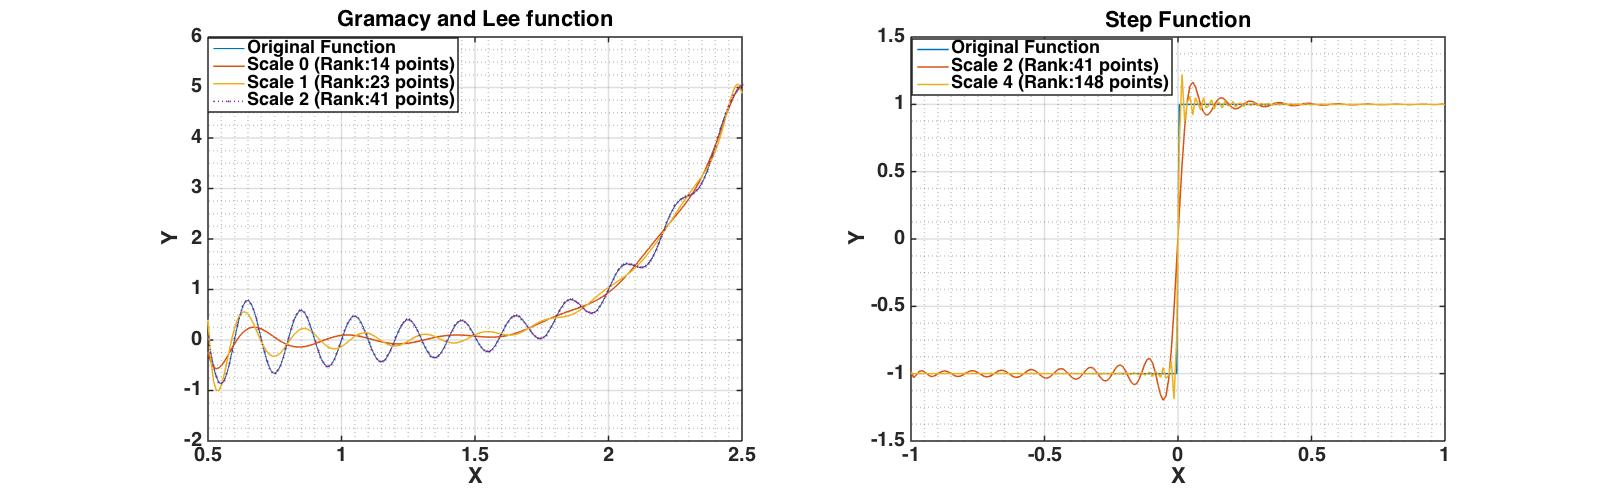
\includegraphics[width=5in]{fig3.jpg}
	\caption[Optional caption]{Prediction from sparse data (a):Gramacy and Lee function (b) Step function}
	\label{fig3} %% for referencing the figure later on
\end{figure}




\section{Results}

Following the testing procedure described in the previous section, here we will present and describe the results obtained after the implementation of our multiscale/multiresolution approach on the test function and the gravity data. 



\begin{figure}[]  % H because we want our figure to stay here
	\centering
	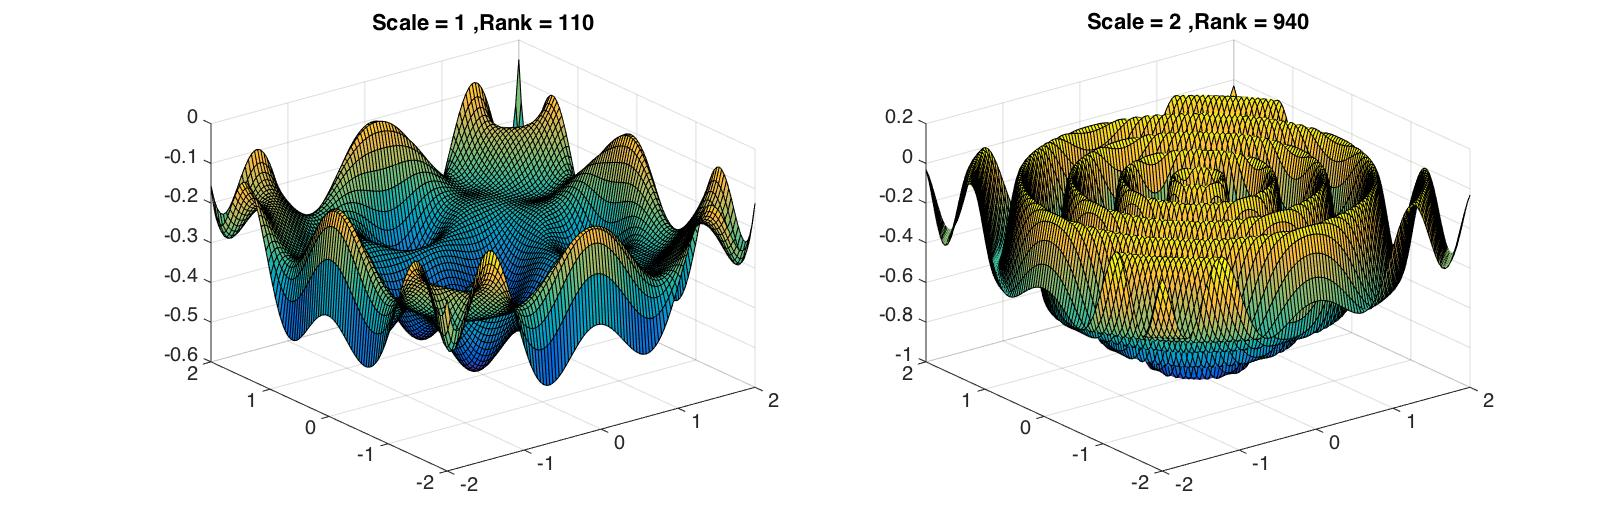
\includegraphics[width=4in]{fig_wave.jpg}
	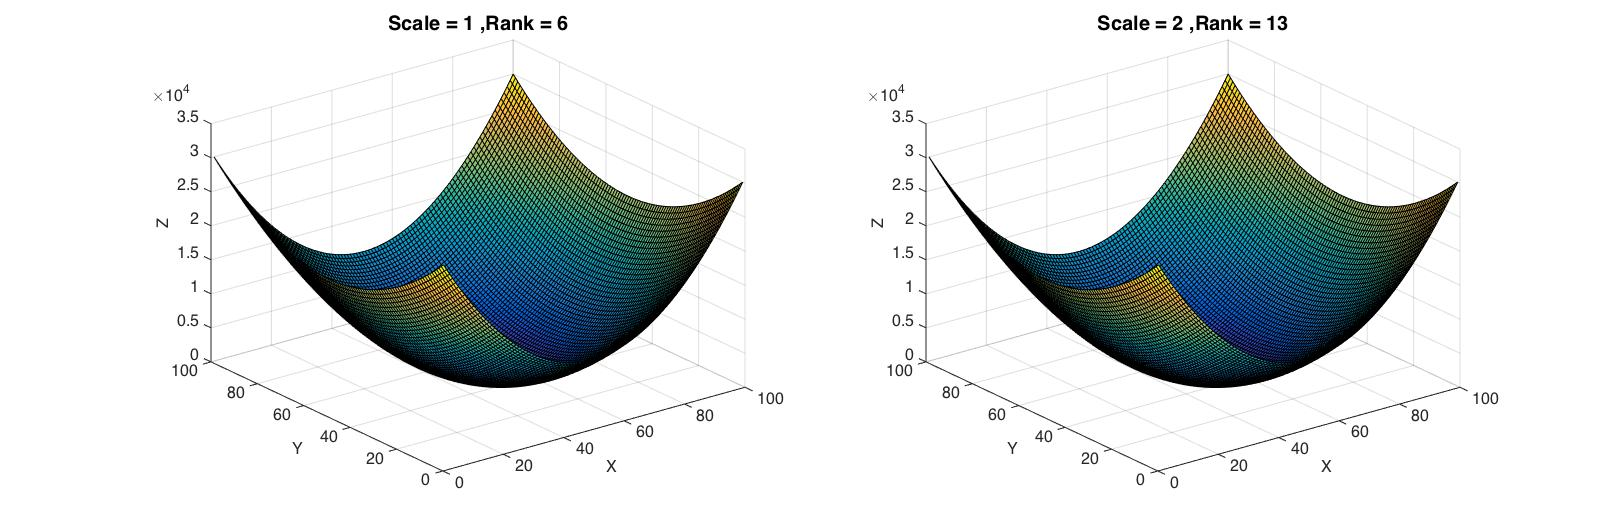
\includegraphics[width=4in]{fig_boha.jpg}
	\caption[Optional caption]{Prediction from sparse data: The drop Wave function (Top row) Bohachevsky function (Bottom row)}
	\label{fig4} %% for referencing the figure later on
\end{figure}





\subsection{Constant Resolution ($\alpha$)}

For this first part, the resolution ($\alpha$) is fixed at 0.5 and scale built into ($\epsilon$) is varied during the analysis. Figure \ref{fig3} shows the results for the first two test functions. For Gramacy and Lee function, it can be seen that as the scale is increased, $\epsilon$ is reduced and therefore the rank of the kernel is increased and thus more and more are chosen for the sparse representation. It is found that around 41 points are able to explain the variation in the function. The quantification of the accuracy would be presented in the following subsections. 

For the step function, we employed a similar procedure to find a sparse representation. However, it could be observed that even with 148 of the original 200 points, we can still see the ringing effect at the discontinuity. These fluctuation do not go away even if we use all the original points and construct the basis functions. Therefore for dealing with this we have used the concept of adaptive resolution discussed in the next subsection.

Figure \ref{fig4} show the effect of variation of scales and predicting the underlying function from the sparse representation obtained at different scales for the Wave and Bohachevsky function. The top two figures show that when the number of critical points chosen are increased from 110 to 940 (as a result of increment in scale) for the drop wave function, the predicted function from this sparse representation becomes highly accurate as shown in Table \ref{tab1}. For the Bohachevsky function, the compression possible is very extreme and it able to reproduce a close approximate of the original function with just 13 points. Based on the behavior of these test function, the observation points chosen at strategic locations at different scales have been shown in Figure \ref{fig5}. Here the blue points show the original points available and the chosen points for sparse representation are circled in red. For the 2 dimension functions, the points are shown in the XY plane instead of the 3 dimension plane for better clarity






\subsection{Adaptive Resolution ($\alpha$)}

Due to Gibbs phenomenon, the prominent ringing effect in the modeling of the step function has motivated us to use the second degree of freedom in the covariance kernel. This is done by adaptively varying the resolution parameter over the entire domain at each scale. In order to do so, at each scale, the resolution at a point is defined as a function of its distance from the point of discontinuity. Therefore, one piece of information which goes into modeling of discontinuity through this method is that the point of discontinuity should be approximately known. The precision with which the modeler knows the location of discontinuity, the more accurate would be results. For the results shown in Figure \ref{fig6} (top left quadrant), we used the values of resolution at a point as 0.5 times the distance from the discontinuity at each scale. Therefore, at very close proximity to the discontinuity, alpha would be very small and hence, it will affect a very small region. Thus, this sort of formulation for the resolution ensures that in the limit towards the point of discontinuity, the region of impact of an observation becomes zero and therefore it doesn't cause any ringing or unnecessary fluctuations. This pattern of defining the sparse representation by using an adaptive combination of variation in scales and resolution also leads to a variation in the the pattern in which points are chosen for sparse representation. It could be seen that unlike the top right plot in Figure \ref{fig5}, where points were uniformly chosen, here (plot 1 in top left quadrant of Figure \ref{fig6}), more points are automatically chosen near the discontinuity, so that it can be accurately modeled. The result of prediction from the sparse representation has been shown in plot 2 in this top left quadrant of Figure \ref{fig6}. The fact that ringing effect has almost completely disappeared with just 52 points justifies our use of an adaptive resolution approach. 


\begin{figure}[]  % H because we want our figure to stay here
	\centering
	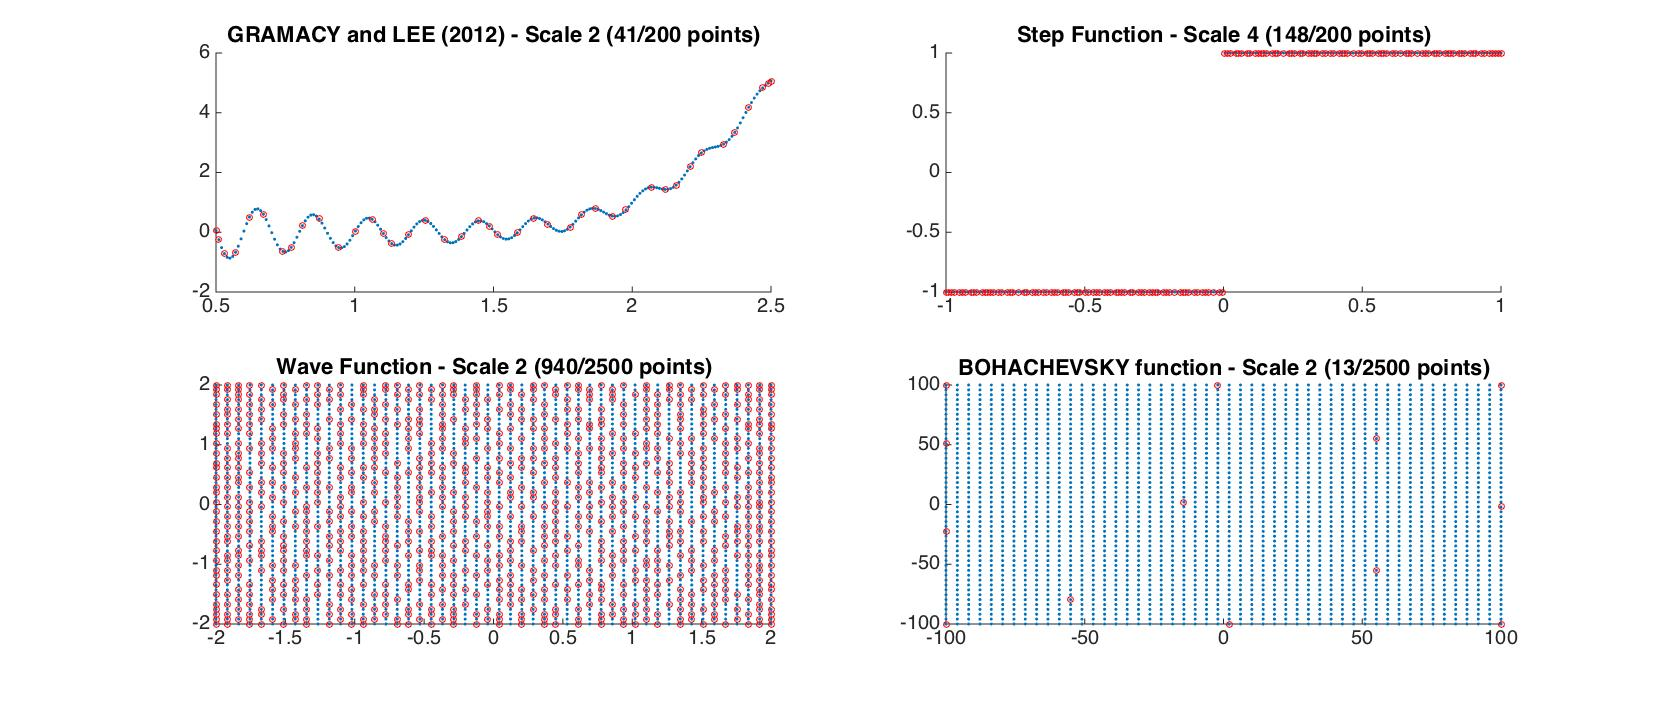
\includegraphics[width=4.3in]{sparse.jpg}
	\caption[Optional caption]{Sparse Representation for the test functions at Relevant scales}
	\label{fig5} %% for referencing the figure later on
\end{figure}



\begin{figure}[]  % H because we want our figure to stay here
	\centering
	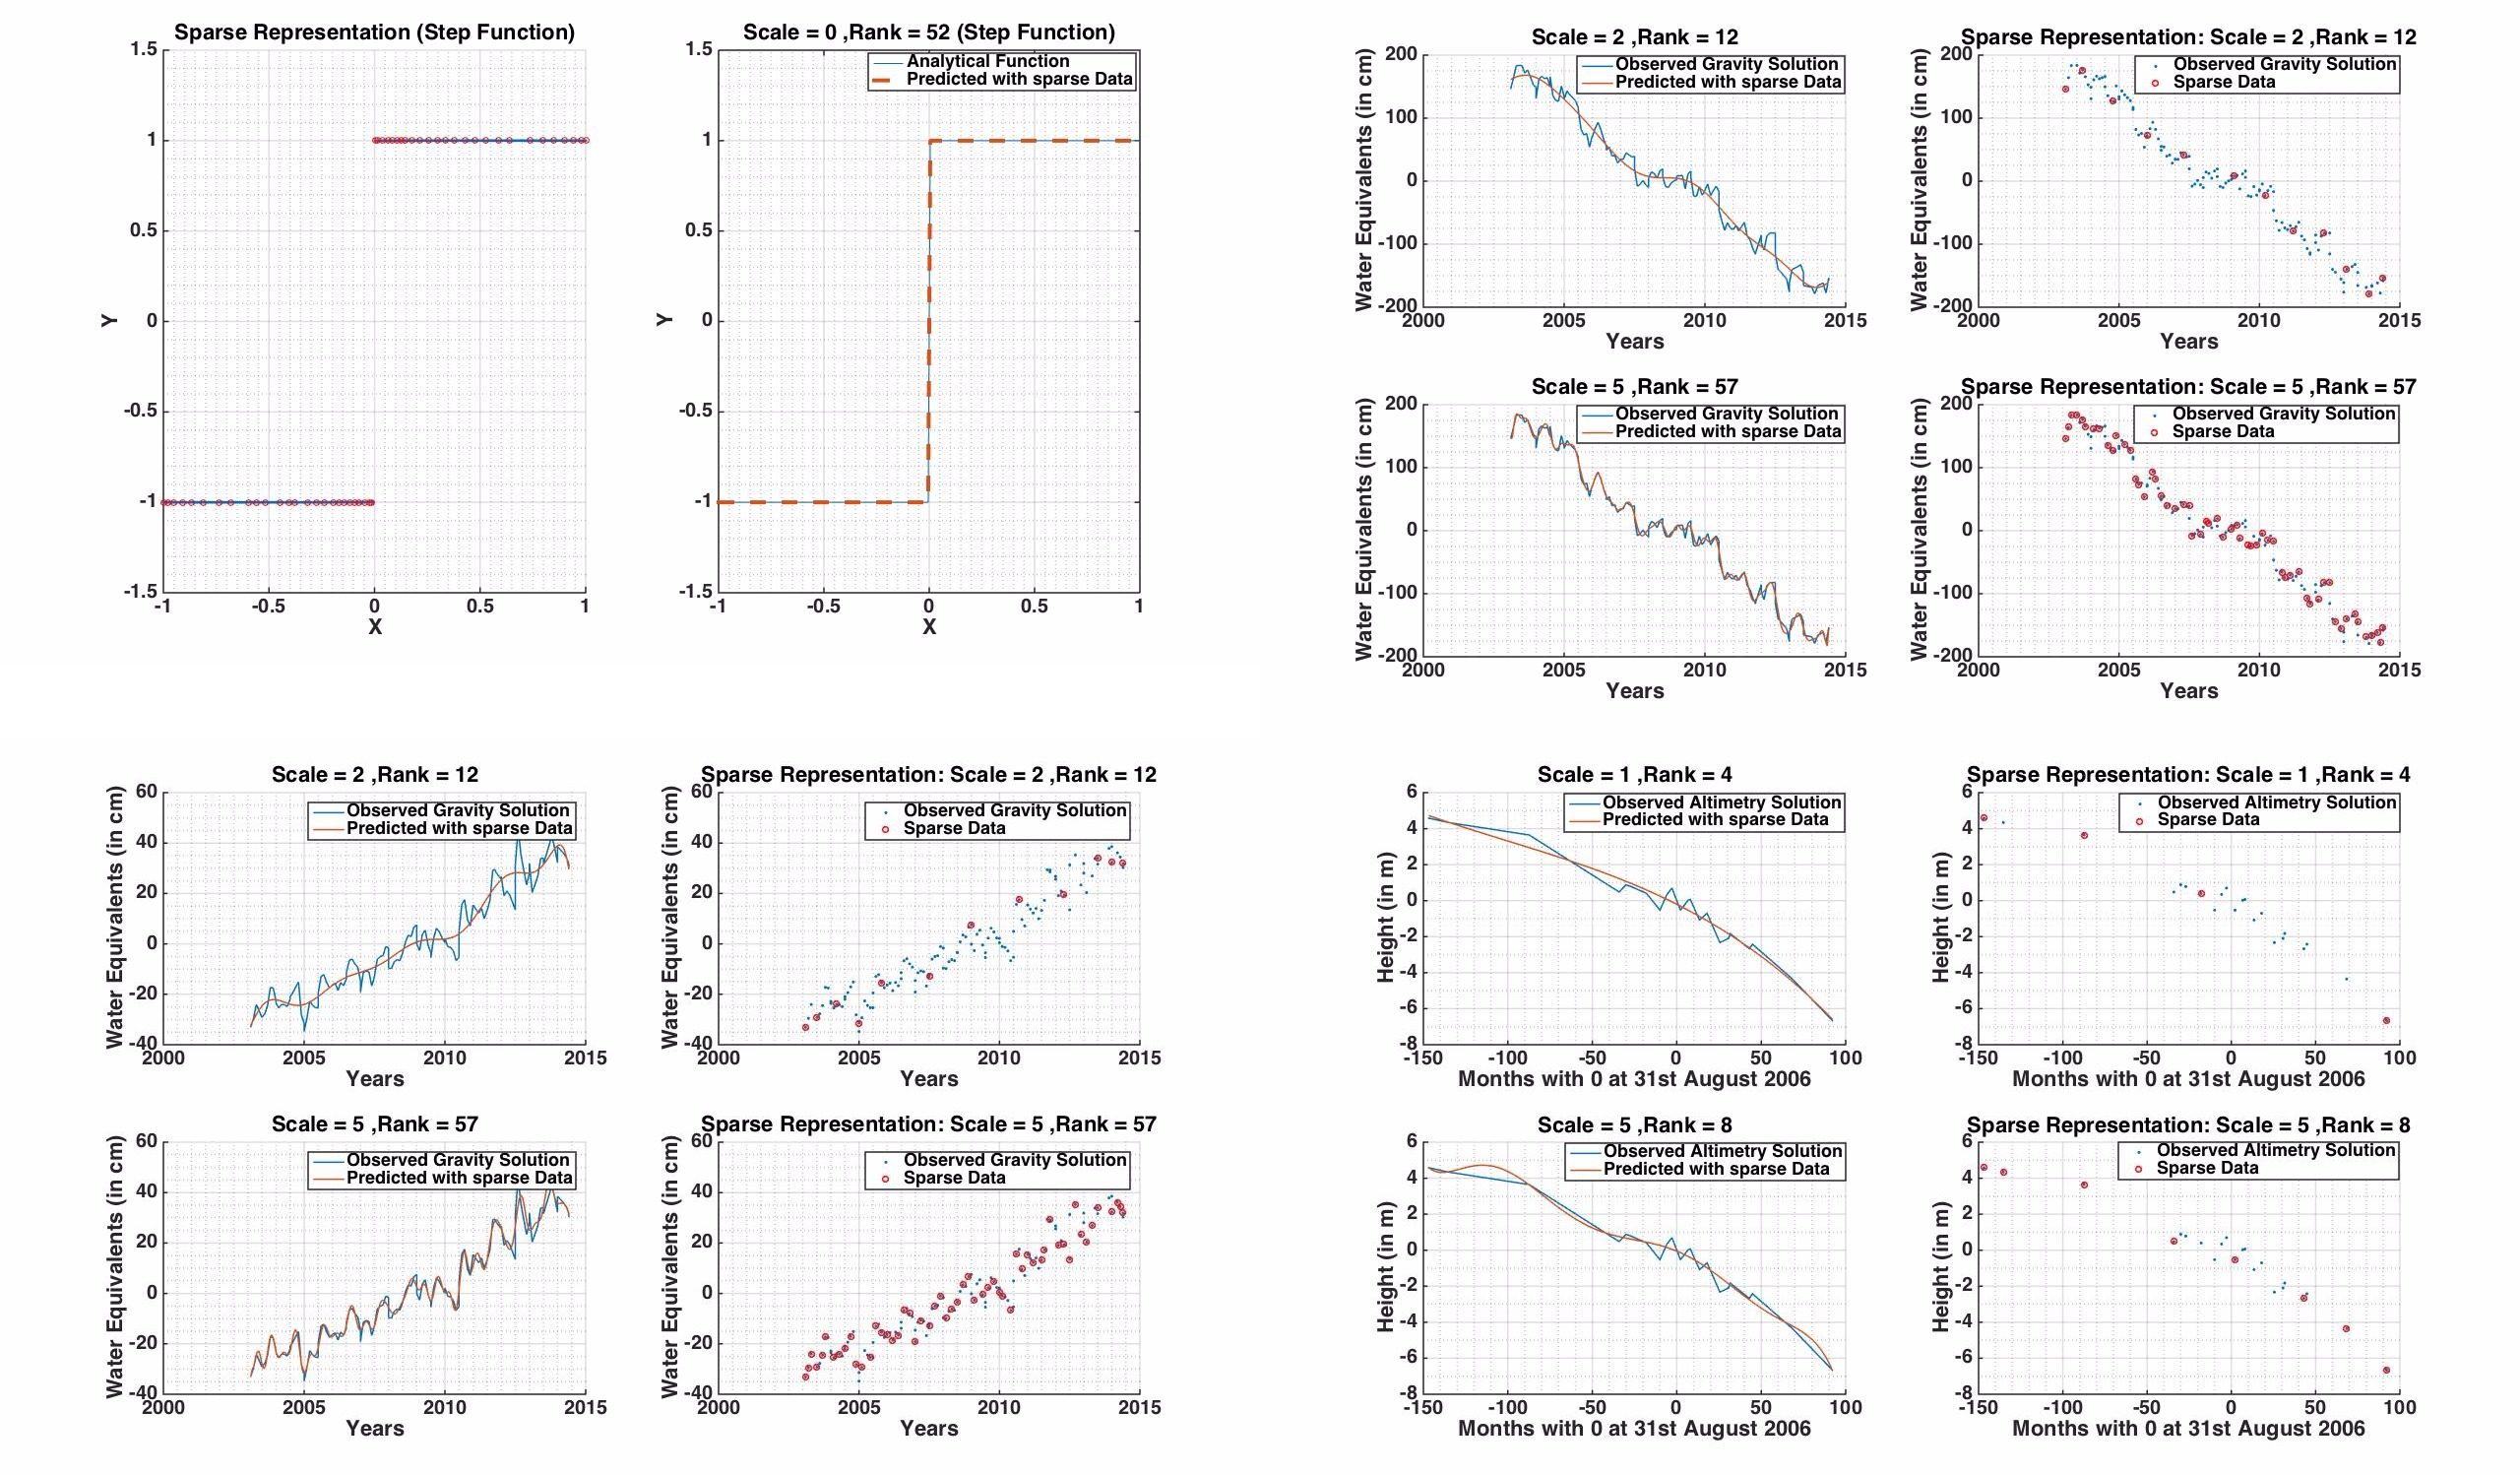
\includegraphics[width=5.9in]{study.jpeg}
	\caption[Optional caption]{\textbf{Top Left quadrant}:  plot 1 shows the sparse representation and plot 2 shows the prediction for step function with variable $\alpha$. \textbf{Top Right quadrant}: Gravity Dataset (Mascon M1). \textbf{Bottom left quadrant}: Gravity Dataset (Mascon M2). \textbf{Bottom right quadrant}: Altimetry Dataset}
	\label{fig6} %% for referencing the figure later on
\end{figure}



\subsection{Accuracy Results}

\begin{table}[htp]
	\begin{centering}
		\begin{tabular}{lrrrrrrrr}
		\hline
		Test Function            &Number of originally &Scale  &Number of Points &RMSE of 20  \\
		                      &sampled point  & &in Sparse Rep. &random pred. points \\
		\hline
		Gram. \&  Lee      &200 &2 &41 &2.85e-05 \\
		Step (adaptive $\alpha$)      &200 &0 &52  &6.10e-07 \\
		The Drop Wave             &2500 &2 &940 &5.83e-05\\
		Bohachevsky      &2500 &2 &13 &7.6009 \\

		\hline
		\end{tabular}
		\caption{Accuracy in terms of RMSE at 20 prediction points through the sparse representation}
		\label{tab1}
	\end{centering}
\end{table}



Table \ref{tab1} shows the root mean square error of prediction at 20 random points chosen in the respective domains. It could be seen that at the scales discussed in Figures \ref{fig3}  and \ref{fig4}, the prediction accuracy is very good for all the test functions (evident from the small RMSE). Here the RMSE of the Bohachevsky function is found to be very high relatively. This is due to the nature of the function which produces values of the order 4 as shown in Figure \ref{fig1}. 





\subsection{Practical Application}

For the gravity dataset, the sparse representation of the time series at Mascon M1 has been shown in the plots in top right quadrant of Figure \ref{fig6}. Here, the right hand side plots show the points which where chosen for sparse representation at different scale. The corresponding left hand side plots show the the prediction of the underlying function through these sparse datasets. It can be seen that as scale is increased the prediction is becoming accurate. Here, the original number of points available is 127 from which 57 points have been chosen at scale 5. This kind of sparse representation also helps as it may also help in noise removal as seen in the bottom left plot in this top right quadrant of Figure \ref{fig6}. Similar results have been obtained for Mascon M2 (shown in bottom left quadrant of Figure \ref{fig6}).

For the altimetry dataset we have just shown it for one coordinate at the edge of the icesheet shown in the rightmost plot in Figure \ref{fig2}. Here also we have obtained similar results where we are able to generate the sparse representation from the original dataset (this time series contains 23 time instances). Here it could be seen that with around 8 points at scale 5 the algorithm is able to capture most of the variability in the dataset (bottom right quadrant of Figure \ref{fig6}). However, at the starting time instances, due to very sparse sampling, the fit is not very accurate as there is clear lack of information during the starting months.

\section{Concluding Remark} 

In this research we proposed a strategy in which we can compress a dataset by removing all the unnecessary observations and retaining only the valuable observation instances. The approach as discussed in our previous work \cite{patra2016multilevel} is based on a QR matrix decomposition procedure which identifies the observation instances with maximum amount of information (through the decomposition of the covariance kernel) and uses them along with the kernel specified as a sparse representation for the original dataset. Then this sparse representation could be used to predict the original function at any time as required. The application of the approach has been shown on 4 analytical functions along with two real datasets from the geophysical domain. 

The approach is shown to be highly useful in a variety of settings. However, there are still several ways in which it could be improved for making the implementation more practical. Firstly, although we introduced a distributed implementation of the approach in \cite{patra2016multilevel}, still improvements have to made there for better scaling. Due to the vast availability of literature in Kernel methods, there may be some way to capture the covariance between the data points in an even better way. Comparison with existing data compression approaches related to Fourier representations can also lead us to better hybrid approaches. Some future work can also  done in extending the approach to the spatio-temporal modeling domain.



%% References

\bibliographystyle{plain}
\bibliography{paper}









































%------------------------------------------------------------------------------
\end{document}

% EOF
